\graphicspath{{../03Mathematics/pics/}}

\chapter{Mathematics}\label{ch:Mathematics}

\lettrine[lines=2]{\color{darkocre}I}{n} the previous chapter we
learned about numbers and various relations between them. As a
particular class of relations we discussed functions. We introduced
\emph{binary} and \emph{unary} functions and different ways
functions can be combined (\emph{composed}) to produce new
functions. We also learned
that functions can be
represented in various ways and that none of those different
representations defines
the concept of function completely. Each representation of a function
highlighted some important aspect of it.

Vectors, which will be introduced in this chapter, also allow
different representations. We will start with a particular model of
vector quantities --
\emph{arrows}\index{Arrows}. It is important to
remember that while this model illustrates the concept of vectors, it
does not define vectors completely. In other words, arrows are
particular examples of vectors, but vectors are more that just
directed line segments.

To arrive at the definition of vectors we must
explore their properties more fully. This will be the goal of current
chapter.

\section{Arrows}

To arrive at the idea of vectors we will start with simple geometrical
objects -- arrows in a plane, as illustrated in the Figure \ref{fig:arrowsSpace}.

\begin{SCfigure}%[htbp]
  %\centering
  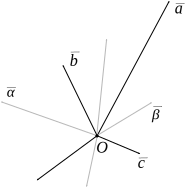
\includegraphics[scale=1.0]{arrowsSpace}
  \caption{Set of arrows starting at the same origin point $O$. All
    imaginable arrows taken as one set form the arrow space
    $\overset{\Rightarrow}{A}$.}
  \label{fig:arrowsSpace}
\end{SCfigure}

Symbolically, we will denote vectors by placing an arrow over letters:
\[
\vec{a}\,,\vec{b}\,,\vec{c}\,,\ldots\,,\vec{\alpha}\,,\vec{\beta}\,.
\]
The length of an arrow $\vec{a}$ is denoted by the same letter
without an arrow:
\[
\btc{length}\,\vec{a} = a\,.
\]

The set of all possible arrows -- called \emph{arrow space} (or
\emph{vector space}\index{Vector!space}) -- we will denote as
\[
	\overset{\Rightarrow}{A} = \lbrace \vec{a}\,,\vec{b}\,,\vec{c}\,,\ldots\,,\vec{\alpha}\,,\vec{\beta}\,\ldots \rbrace\,.
\]
Diagrammatic representation of the set of arrows is given in the
Figure \ref{fig:arrowsSpaceDiagram}.
\begin{SCfigure}%[htbp]
  %\centering
  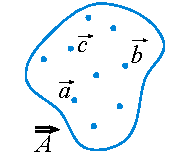
\includegraphics[scale=1.0]{arrowsSpaceDiagram}
  \caption{All arrows, considered as unified collection of objects of
    similar nature, can be viewed as a mathematical set. Each arrow is
    an element of this set, denoted as a point.}
  \label{fig:arrowsSpaceDiagram}
\end{SCfigure}

%\begin{tcolorbox}[colback=white!85!ocre, title=Functions on arrows]
\begin{mybio}{Functions on Arrows}\\
The function $\btc{length}$ is a unary function that accepts arrows as input
(argument) and returns a numeric value -- the lengths of the arrow.

On the level of sets, the $\btc{length}$ function \emph{maps} the set
of all vectors into the set of real numbers:
\[
\overset{\Rightarrow}{A}\overset{\btc{length}}{\longrightarrow}\mathbb{R}\,.
\]

In the next chapter we will encounter other types of functions on arrows. Some of
them will return numbers, like $\btc{length}$ does, and others will return
arrows, mapping \emph{arrow space} into its own copy:
\[
\overset{\Rightarrow}{A} \longrightarrow \overset{\Rightarrow}{A}\,.
\]
\end{mybio}

\begin{SCfigure}%[htbp]
  %\centering
  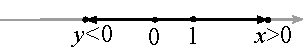
\includegraphics[scale=1.0]{arrowsNumberLine}
  \caption{Real numbers\index{Numbers!real} can be represented by
    arrows oriented along a
    fixed line -- \emph{number line}.}
  \label{fig:arrowsNumberLine}
\end{SCfigure}

%\begin{tcolorbox}[colback=white!85!ocre, title=Arrows and Numbers]
\begin{mybio}{Arrows and Numbers}
Arrows in a plane include, in some sense, the notion of
numbers. Indeed, as shown in the Figure \ref{fig:arrowsNumberLine},
real numbers may be represented as points on a line -- number
line. Positive numbers correspond to arrows pointing to the right of
the origin (number zero), negative numbers correspond to the arrows
directed to the left.
\end{mybio}
%\end{tcolorbox}


\section{Algebra of Arrows}
Next, we will establish similarities between arrows and numbers by
exploring possible \emph{algebraic operations} on vectors.


\subsection{Combining Arrows}

Two arrows can be \emph{combined}\index{Arrow!addition} in a natural
way to yield the third arrow.
Using either the head-to-tail approach or a parallelogram method,
the vectors \textbf{$\vec{a}$} and $\vec{b}$ can be combined
graphically, as illustrated in Figure \ref{fig:arrowsAddition}.

\begin{figure}[htbp]
  \centering
  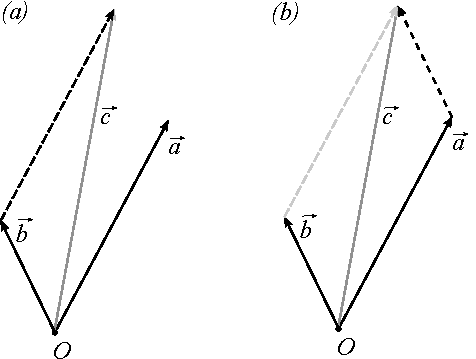
\includegraphics[scale=1.0]{arrowsAddition}
  \caption{Two arrows can be combined to produce new
    arrow. One of the simplest way to do this is to arrange two arrows
  ``tail-to-tip''. This operation is called \emph{addition of arrows}:
  $\vec{a}+\vec{b}=\vec{c}$.}
  \label{fig:arrowsAddition}
\end{figure}


\section*{Chapter Highlights}
{\setstretch{1.5}\chhc
  \it
  \small
\begin{itemize}
\item Arrows in a plane provide a simple model for vectors.
\item Arrows can be manipulated in ways analogous to numbers: Two arrows
  be added, an arrow can be ``scaled'' (stretched or compressed). Arrows form
  an algebra.
\item Basis is an extremely important concept. Basis is a set of
  objects (arrows) that can be used to ``build'' all other similar
  objects (arrows). At the same time, basis can not be used to build
  itself -- basis arrows are independent.
\item Basis can be chosen in infinite number of ways. There is no
  special basis. Different bases might be useful for different
  problems.
\item Given a basis, arrows can be specified by writing their
  components (using index notation) relative to the basis.
\item Einstein's summation rule is very useful for manipulating
  expressions involving components of arrows.
\item The exact values of the arrow's components depend on the
  basis. Changing the basis changes the values of components, while
  the arrow remains the same. This is one of defining properties of
  vectors.
\item When basis is changed, components of the same arrow transform in a
  very specific way. Depending on exact form of transformation, we can
  speak of two kind of vectors: contravariant and
  covariant. Arrow-like vectors are example of contravariant vectors.
\end{itemize}
}
